\section{Grafiken einbinden}

% das hier ist eine willkürliche Skalierung
%\includegraphics[scale=0.1]{../img/cat.jpg}
% wenn eine Grafik im selben Verzeichnis liegt,
% dann muss man nur den Namen angeben: cat (ohne Dateiendung)
%\includegraphics[]{cat}

% Nachteil: unübersichtlich bei mehreren Grafiken

% das hier ist nicht so schön, weil verzerrt
%\includegraphics[width=1cm, height=5cm]{../img/cat.jpg}

% textweite, texthöhe
% ist uns aber zu viel zu hoch
%\includegraphics[width=\textwidth, height=\textheight]{../img/cat.jpg}

% textweite, texthöhe
% TODO: ist uns aber zu viel zu hoch, deshalb verkleinern wir
%\includegraphics[width=\textwidth, height=\textheight]{../img/cat.jpg}

% dynamische Größenanpassung mit beibehaltenen Verhältnissen
%\includegraphics[width=0.8\textwidth,
%height=0.2\textheight,
%keepaspectratio]
%{../img/cat.jpg}

%\begin{figure}
%\end{figure}

\section{Katzen mit Labeln}

\begin{figure}[h!] % figure mit platzierungsoptionen
    \begin{center}
\includegraphics[width=0.8\textwidth,
    height=0.2\textheight,
    keepaspectratio]
    {../img/cat.jpg}
    \caption{Zwei flauschige Katzen.}
    \label{fig:cat}
    \end{center}
\end{figure}

\begin{figure}[h!] % figure mit platzierungsoptionen
    \begin{flushleft}
        \includegraphics[width=0.8\textwidth,
        height=0.2\textheight,
        keepaspectratio]
        {../img/cat.jpg}
        \caption{Zwei flauschige Katzen.}
        \label{fig:cat-left}
    \end{flushleft}
\end{figure}

\begin{figure}[h!] % figure mit platzierungsoptionen
    \begin{flushright}
        \includegraphics[width=0.8\textwidth,
        height=0.2\textheight,
        keepaspectratio]
        {../img/cat.jpg}
        \caption[Katzen-rechts]{Zwei flauschige Katzen.}
        \label{fig:cat-right}
    \end{flushright}
\end{figure}

Katzen wie in \ref{fig:cat} sind flauschig.
Katzen wie in \ref{fig:cat-left} sind links und flauschig.
Katzen wie in \ref{fig:cat-right} sind rechts und flauschig.


\subsection{Optionen}
\begin{itemize}
     \item \texttt{scale=WERT}: skaliert eine Grafik, Angabe von \texttt{WERT} ist sinnvoll und schön im (geschlossenen) Intervall $[0,1]$ aber es gehen auch beliebige Werte. Andere Angaben sind auch möglich.
     \item wir können auch die Breite und die Höhe bestimmen: \texttt{width=WERT} und \texttt{height=WERT}.
     \item \texttt{WERT} kann aber auch die Ausgabe eines Markos sein.
\end{itemize}

% viel mehr: <https://en.wikibooks.org/wiki/LaTeX/Floats,_Figures_and_Captions>


\clearpage
\listoffigures
